\documentclass[12pt]{article}
\usepackage{geometry}
\usepackage{amsfonts, epsfig}
\usepackage{amsmath}
\usepackage{wrapfig} % for wrapping text around figures and tables
\usepackage{graphicx}
\usepackage{fancyhdr}
\usepackage{booktabs} % for better table rules
\usepackage{caption} % to customize caption format
\usepackage{linegoal} % for determining the remaining width of the line
\usepackage[backend=biber, sorting=none]{biblatex}

% reference file
\addbibresource{report.bib}

\geometry{
    left=20mm,
    right=20mm,
    top=20mm,
    bottom=20mm
}

% header and footer
\makeatletter
\def\@oddhead{\parbox{\textwidth}{\raggedright\sffamily\underline{\texttt{Question 1 - Visualization and analysis of the Palmer penguin dataset}} \hfill \thepage}}
\def\@oddfoot{\parbox{\textwidth}{\raggedright\footnotesize\texttt{emamtm0067.github.io} / \texttt{ematm0044.github.io}}}
\makeatother

% Redefine the table and figure formats to bold
\captionsetup[table]{labelfont=bf}
\captionsetup[figure]{labelfont=bf}
\captionsetup{font=small}

\begin{document}
\begin{center}
\subsection*{Q1 - Visualization and analysis of the Palmer dataset}
\end{center}

\begin{wraptable}{r}{0.5\textwidth} % {alignment}{width}
  \small
  \begin{center}
  \vspace{-1.5\baselineskip} % Remove space before the table
  \setlength{\abovecaptionskip}{5pt}
  \setlength{\belowcaptionskip}{5pt}
  \fontsize{10}{10}\selectfont % Change font size here
  \begin{tabular}{l|l|l}
  Attribute&Type&Values in the dataset\\
  \hline
  species&categorial&Adelie, Chinstrap, Gentoo\\
  island&categorial&Torgersen, Biscoe, Dream\\
  bill length&numerical&32.1mm - 59.6mm\\
  bill depth&numerical&13.1mm - 21.5mm\\
  flipper length&numerical&172mm - 231mm\\
  body mass&numerical&2700g - 6300g\\
  sex&categorial&Male, Female
  \end{tabular}
  \vspace{-1.5\baselineskip} % Remove space before title
  \end{center} 
  \caption{Attributes of the Palmer penguin dataset}
  \vspace{-1\baselineskip} % Remove space after the table
  \label{tab:dataset}
\end{wraptable} 

\noindent
The Palmer penguin dataset consists of 344 records of the physical attributes of three species of penguin 
living on three islands in Antarctica (Table~\ref{tab:dataset}) \cite{PM}. 
In this report, consideration is given to data cleaning and preparation, 
the dataset is explored through visualization and analysis is carried out 
to compare the accuracy performances of a small number of AI approaches. 

\vspace{\baselineskip}
\subsection*{Data cleaning - missing values, standardization and data imbalance}

\begin{wrapfigure}{r}{0.5\textwidth} % {alignment}{width}
  \centering
  \vspace{-0.5\baselineskip} % Remove space before the table
  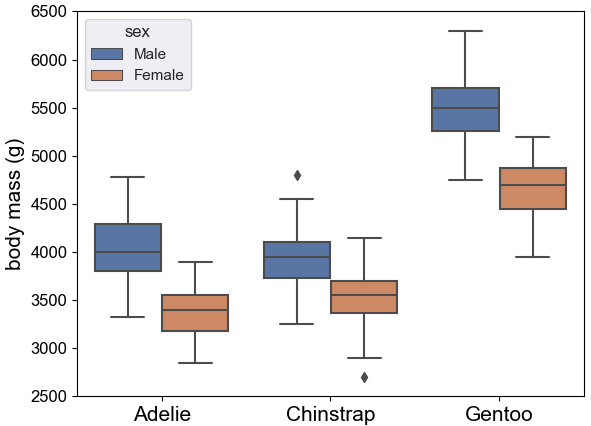
\includegraphics[width=0.48\textwidth]{sex.png} % Adjust the width as needed
  \vspace{-0.5\baselineskip} % Remove space before title
  \caption{All numerical features show a significant statistical difference between the male and female measurements, as seen in the body mass boxplot above. Shown are median values, Q1 and Q3 quartiles, as well as outliers that are outside the range Q1-1.5IQR to Q3+1.5IQR, where IQR=Q3-Q1.}
  \vspace{-0.5\baselineskip} % Remove space before title
  \label{fig:sex}
\end{wrapfigure}   

Two of these records can be deleted immediately as they are missing 
values for all of the numerical attributes and the sex feature 
and any imputation is unlikely to be reliable. 
The remaining nine records have no value only for the sex attribute. 
As can be seen in Figure~\ref{fig:sex}, the physical attributes of the male and female of each species 
are statistically different and so it is reasonable to consider assigning a sex 
to those records missing this attribute. Following standardization, 
a Shapiro-Wilk test was performed to confirm each numerical attribute exhibits a normal distribution \cite{shapiro1965analysis} 
and Z-tests were performed to assess separately both the 
hypothesis that the missing sex value is male and that it is female \cite{freedman2007statistics}. 
It was found that two of the records could be imputed as male and three as female 
and these were then retained in the dataset. 
The remaining four records were removed from the dataset. 
The cleaned dataset consisted of 338 records made up of 147 Adelie penguins 
(74 male, 73 female), 68 Chinstrap penguins (34 male, 34 female) and 123 Gentoo penguins (62 male, 61 female).

A number of the methods applied in this work involve distance measures 
and so may be biased in favour of features with smaller standard deviations \cite{hastie2009elements}. 
This bias can be removed by standardizing the four numerical attributes independently 
(to give zero mean and unity standard deviation). 
Standardization uses only the statistics of training sets, 
but standardization is also applied to test sets. If a dataset is imbalanced, 
AI approaches may be biased in predicting classes that are more commonly found in the training data. 
The Palmer penguin dataset is somewhat imbalanced, 
with the number of Chinstrap records being around half of that of either Adelie or Gentoo, 
which are present in similar numbers. 
The importance of imbalance depends on the analysis method applied. 
It is known that all the methods adopted in the current work are generally little affected by imbalanced data \cite{he2009learning} 
and so no modifications were made to reduce imbalance.

\vspace{\baselineskip}
\subsection*{Visualization of the dataset}

\begin{wrapfigure}{r}{0.5\textwidth} % {alignment}{width}
  \centering
  \vspace{-0.5\baselineskip} % Remove space before the table
  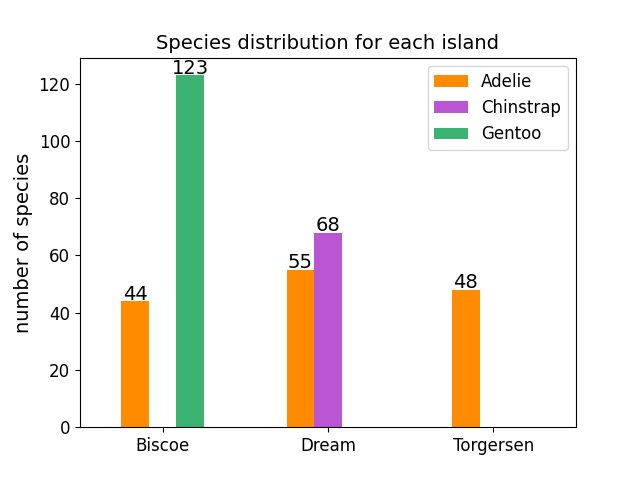
\includegraphics[width=0.48\textwidth]{islands.png} % Adjust the width as needed
  \vspace{-0.5\baselineskip} % Remove space before title
  \caption{All numerical features show a significant statistical difference between the male and female measurements, as seen in the body mass boxplot above. Shown are median values, Q1 and Q3 quartiles, as well as outliers that are outside the range Q1-1.5IQR to Q3+1.5IQR, where IQR=Q3-Q1.}
  \vspace{-0.5\baselineskip} % Remove space before title
  \label{fig:islands}
\end{wrapfigure}

Figure Figure~\ref{fig:islands} shows the species distribution across the three islands in the study. 
Chinstrap and Gentoo penguins are found only on one island, so island is a potential confounding factor, 
possibly affecting physical characteristics due to environmental factors (such as predators or food supply). 
A Shapiro-Wilk test was used to confirm that the numerical features of the Adelie penguins (that are found on 
all the islands) are normally distributed and an ANOVA test confirmed that their physical characteristics are not significantly influenced by the island inhabited. 
Consequently, it was considered unlikely that the island is a confounding factor in the dataset.




You can write in \textbf{bold}, or \textsl{italics} or \texttt{true
  type}, often the latter is used for specific commands or libraries in a
programming language, as in `I used \texttt{numpy} v1.23.4 to\ldots'. Notice the use of the left quote symbol found in the top left of the keyboard to get the left quote. There is also blackboard bold often used for things like $\mathbb{R}$ for real numbers and there is calligraphic for fancy things like $\mathcal{L}$ but this is becoming increasing irrelevant to what you are likely to need! 




\printbibliography


\end{document}
